\chapter{Organisation} \label{organisation}
\section{Planning} \label{planning}
The planning presented in this chapter is representative of the structure presented in chapter \ref{methodology}, the various steps and results are represented in both the tabular representation [Table \ref{tab:time}] as well as the Gantt-chart [Figure \ref{fig:gantt}], albeit under slightly altered names. The Gantt chart provides a more detailed overview of the various steps including time for writing and correction by supervisors. Leading in the configuration of the planning have been the presentation moments [or Ps]. P3 has been used as a subdivision between the work from block B and C as described in the previous chapter. This to ensure sufficient time before the final presentations for potential slight adjustments in the progress. \\
Biweekly meetings have been agreed upon with the supervisors; supplemented with weekly updates when necessary. This to ensure progress and to facilitate the completion of the research in the remainder of the 2017-2018 academic year. 

\begin{table}[h]
	\centering
\begin{tabular}{llr}
	\toprule
	Task & \multicolumn{2}{c}{Time allocated} \\
	\cmidrule{2-3}
	& Start week & Duration in weeks \\
	\midrule
	Framework development		& Week 48 \hfill [2.3]   & 6   \\
	Methods selection			& Week 48 \hfill [2.3]   & 6   \\
	Data preparation			& Week 5  \hfill [2.10]   & 4  \\
	Methods assessment			& Week 7 \hfill  [3.1]    & 5   \\
	Results assessment			& Week 10 \hfill [3.4]   & 3   \\
	Method development			& Week 10 \hfill [3.4]   & 6   \\
	Validation					& Week 16 \hfill [3.10]   & 3   \\
	Visualisation				& Week 17 \hfill [4.1]   & 2   \\
	\bottomrule
\end{tabular}
	\caption{Planned tasks and allocated time, TU Delft academic weeks between brackets. [From: own work]}
	\label{tab:time}
\end{table}

\begin{figure}[h]
	\centering
	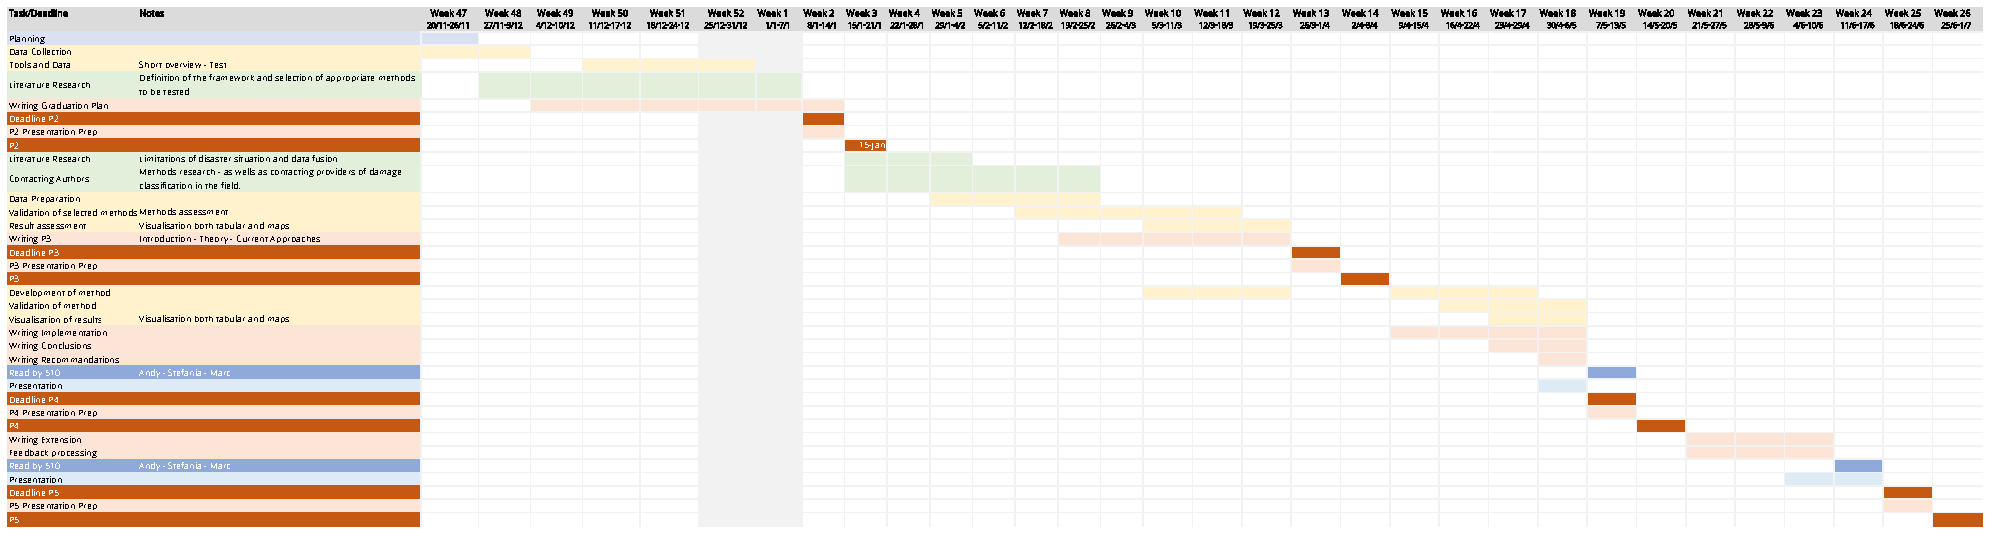
\includegraphics[width=0.9\textwidth]{figs/gantt.png}
	\caption{Gantt chart representation of the planning - full size attached in Appendix \ref{an1} [From: own work]}
	\label{fig:gantt}
\end{figure}